\smalltitle{سوال 2}
\\\noindent
در ابتدا به چند نکته اشاره می‌کنم که لازم بود در کد این سوال رعایت کنم.
در ابتدا برای استفاده از تابع
\lr{pthread\_attr\_setaffinity\_np}
مجبور بودم که در اولین خط برنامه قبل از
\lr{import}ها
خط
\lr{\#define \_GNU\_SOURCE}
را اضافه کنم.
(
\link{https://stackoverflow.com/a/7269859/4213397}{منبع}
)
تابع مذکور به ما اجازه می‌دهد که مشخص کنیم که هر ریسمان بر روی کدام هسته‌های
\lr{CPU}
قابل اجرا باشد.

یکی دیگر از مشکلاتی که وجود داشت نیازمندی به
align
کردن مموری به
\lr{page}های
سیستم بود. بدین منظور که به عنوان مثال در سیستم من که سایز صفحات 4096 بایت است،‌ اول مموری که
به تابع
\lr{mprotect}
داده می‌شود باید بر 4096 بخش پذیر باشد.
بدین منظور من به جای استفاده از تابع
\lr{malloc}
از تابع
\link{https://linux.die.net/man/3/pvalloc}{pvalloc}
استفاده کردم که دقیقا برای همین کار ساخته شده است.

همچنین برای سینک کردن ترد‌ها
(ترد‌های $B$، $C$ و $D$ باید صبر کنند که مموری allocate شود و سپس کارشان را بکنند.)
از \lr{cond var}های \lr{pthreads}
استفاده کردم.

همچنین ترجیح دادم که از
\lr{core}
شماره ۰ استفاده نکنم. این
\lr{core}
ممکن است که برای کار‌های حساس سیستم بیشتر استفاده شود پس صرفا از ۱ شروع کردم.
همچنین مشخص است که برای اجرای این برنامه نیاز به حداقل ۵ هسته داریم!

همچنین در ریسمانی که از مموری می‌خواند، برای اینکه بهینه‌سازی‌های کامپایلر دستور خواندن را کلا
حذف نکند، مقدار عضو‌های آرایه را جمع کرده‌ام و آنرا از تابع
\lr{return}
کردم.

همچنین برای تمامی سوالات یک
\lr{Makefile}
نوشته‌ام که می‌توانید صرفا با زدن دستور
\lr{make}
تمام فایل‌ها را کامپایل کنید. این makefile
را از تمرین درس پردازش چند‌هسته‌ای برداشتم.

همچنین کار دیگری که کردم این است که در یک حلقه به تعداد اولین آرگومان برنامه کار گفته شده
(\lr{allocate} کردن و \lr{protect} کردن)
را انجام می‌دهیم.

حال صرفا کد را کامپایل و اجرا می‌کنیم. در ابتدا مشاهده می‌کنیم که در حالتی که
\lr{write} 
داریم به
\lr{SIGSEGV}
بر می‌خوریم.
(یعنی در حالت ب و ج)
\begin{figure}[H]
    \centering
    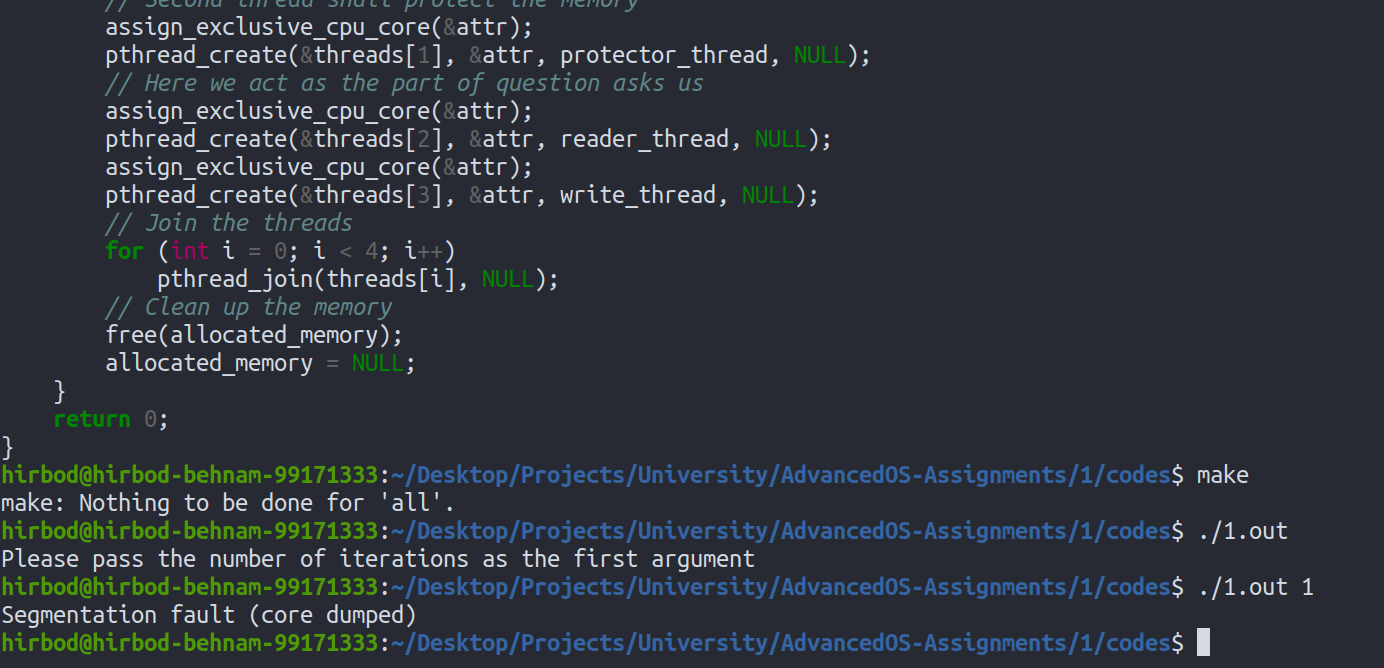
\includegraphics[scale=0.3]{pics/segfault1.png}
    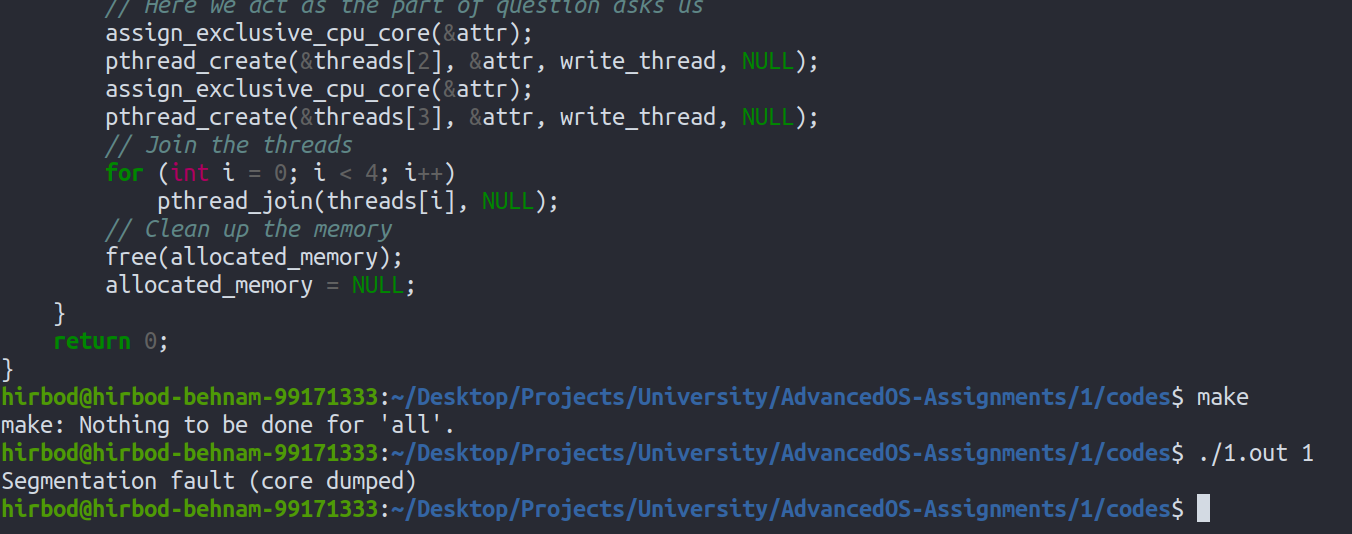
\includegraphics[scale=0.3]{pics/segfault2.png}
\end{figure}

اما در حالتی که دو ترد در حال خواندن هستند مشکلی پیش نمی‌آید.
سپس به کمک \lr{perf}
به ازای تعداد بار‌های مختلف،‌ تعداد
\lr{TLB shootdown}
را اندازه گیری می‌کنیم.
(در ابتدا مقدار مموری allocate شده برابر ۴ کیلوبایت می‌باشد.)
همچنین از دستور زیر برای اجرا کردن و اندازه‌گیری
\lr{TLB shootdown}
استفاده می‌کنیم.
\samplebox{sudo perf stat -e itlb.itlb\_flush,tlb\_flush.dtlb\_thread,tlb\_flush.stlb\_any ./1.out}
\begin{figure}[H]
    \centering
    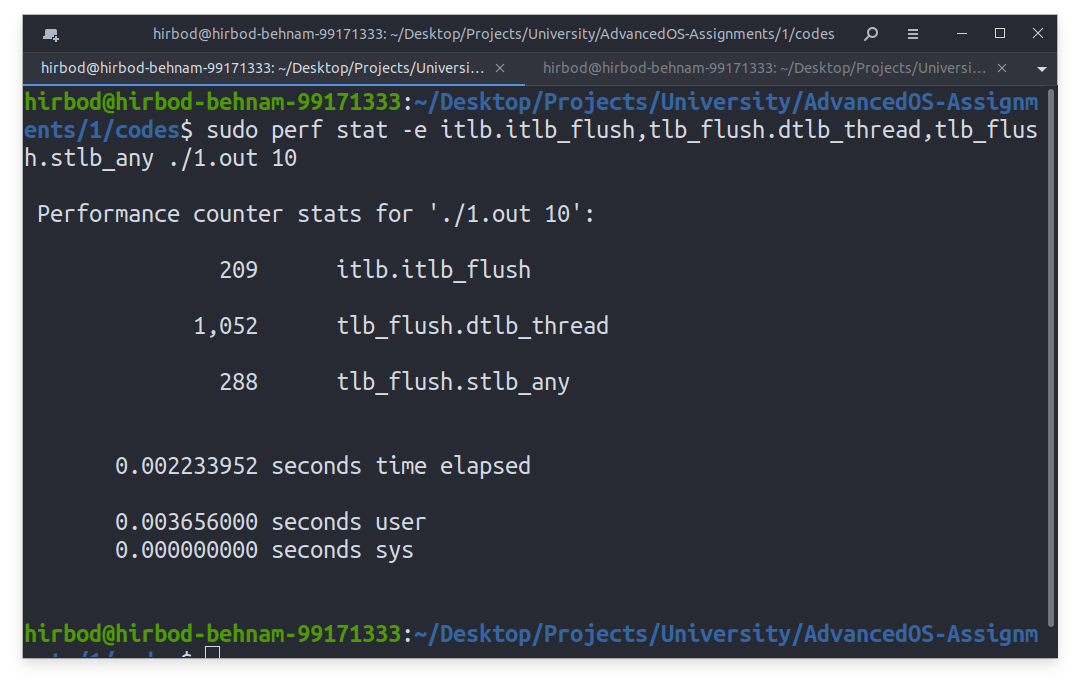
\includegraphics[scale=0.4]{pics/sample-run.png}
\end{figure}
در ادامه نمودار تعداد
\lr{TLB shootdown}
بر حسب آرگومان برنامه را را رسم می‌کنیم.
برای این کار من از یک اسکریپت
\lr{bash}
استفاده کردم که صرفا برنامه را با آرگومان‌های مختلف اجرا می‌کند و یک فایل
\lr{CSV}
بر می‌گرداند. این فایل چهار ستون دارد. ستون اول آرگومان برنامه هست که تعداد دفعاتی است که
عملیات ساخت ترد و حفاظت از مموری انجام می‌شود. بقیه‌ی ستون‌ها به ترتیب تعداد
\lr{flush}های
\lr{instruction TLB}،
\lr{data TLB} و
\lr{secondry TLB}
است. آخرین مورد بین هسته‌های مختلف مشترک است.
(\link{https://stackoverflow.com/q/34437371/4213397}{منبع 1} و \link{https://community.intel.com/t5/Software-Tuning-Performance/Understanding-hardware-performance-counter-event-for-STLB-flush/m-p/985576}{منبع 2})

\begin{figure}[H]
    \centering
    \begin{tikzpicture}
    \begin{axis}
    \addplot table [x=iterations, y=itlb, col sep=comma] {codes/1-stat-4KB.csv};
    \end{axis}
    \end{tikzpicture}
    \caption{\lr{ITLB shootdown} بر حسب آرگومان}
\end{figure}
\begin{figure}[H]
    \centering
    \begin{tikzpicture}
    \begin{axis}
    \addplot table [x=iterations, y=dtlb, col sep=comma] {codes/1-stat-4KB.csv};
    \end{axis}
    \end{tikzpicture}
    \caption{\lr{DTLB shootdown} بر حسب آرگومان}
\end{figure}
\begin{figure}[H]
    \centering
    \begin{tikzpicture}
    \begin{axis}
    \addplot table [x=iterations, y=stlb, col sep=comma] {codes/1-stat-4KB.csv};
    \end{axis}
    \end{tikzpicture}
    \caption{\lr{STLB shootdown} بر حسب آرگومان}
\end{figure}
همان طور که مشخص است به صورت کلی تمامی نمودار‌ها صعودی هستند. ولی چیزی که جالب است
این است که نمودار
\lr{DTLB}
با تقریب کمی خطی است! همچنین مشاهده می‌شود که با اینکه به صورت کلی
\lr{ITLB} و \lr{STLB}
به صورت صعودی بالا می‌روند ولی بعضی وقت‌ها تعداد
\lr{shootdown}ها
نسبت به حالت قبلی کمتر می‌شود.
یکی از دلایلی که برای
\lr{ITLB}
می‌توان آورد، تعداد زیاد
\lr{context switch}
است. همچنین دقت کنید که لزوما تنها این برنامه در حال ران شدن بر روی یک کامپیوتر نیست.
پس هر چه قدر که زمان اجرای برنامه بیشتر باشد، احتمال
\lr{switch out}
شدن ترد بیشتر است. همچنین بخشی از این
\lr{shootdown}ها
\emph{ممکن است}
که برای ساخت و
\lr{join}
کردن ترد‌ها پشت سر هم باشد.

حال برای مقدار یک کیلوبایت آزمایش را انجام می‌دهیم. برای این کار صرفا خط
\lr{\#define ALLOCATED\_MEMORY\_SIZE}
را دست می‌زنیم و جلوی آن
1024
می‌نویسیم. سپس دوباره اسکریپت را اجرا می‌کنیم که فایل
\lr{CSV}
را به ما دهد.
\begin{figure}[H]
    \centering
    \begin{tikzpicture}
    \begin{axis}
    \addplot table [x=iterations, y=itlb, col sep=comma] {codes/1-stat-1KB.csv};
    \end{axis}
    \end{tikzpicture}
    \caption{\lr{ITLB shootdown} بر حسب آرگومان}
\end{figure}
\begin{figure}[H]
    \centering
    \begin{tikzpicture}
    \begin{axis}
    \addplot table [x=iterations, y=dtlb, col sep=comma] {codes/1-stat-1KB.csv};
    \end{axis}
    \end{tikzpicture}
    \caption{\lr{DTLB shootdown} بر حسب آرگومان}
\end{figure}
\begin{figure}[H]
    \centering
    \begin{tikzpicture}
    \begin{axis}
    \addplot table [x=iterations, y=stlb, col sep=comma] {codes/1-stat-1KB.csv};
    \end{axis}
    \end{tikzpicture}
    \caption{\lr{STLB shootdown} بر حسب آرگومان}
\end{figure}
همان طور که مشاهده می‌شود،‌ تفاوت آنچنانی بین شکل‌های ۱ تا ۳ و ۴ تا ۶ وجود ندارد.
دلیل این موضوع می‌تواند این باشد که صرفا به ازای هر
\lr{mprotect}
یک
\lr{TLB shootdown}
داریم و از آنجا که سایز صفحه‌ی سیستم‌عامل من
۴۰۹۶ بایت است، پس مموری
\lr{allocate}
شده در دو حالت در یک صفحه قرار می‌گیرند و عملا رفتار
\lr{mprotect}
یکسان می‌شود بین دو حالت.

در انتها نیز حالات
الف و ب را دوباره بررسی می‌کنیم.
\begin{figure}[H]
    \centering
    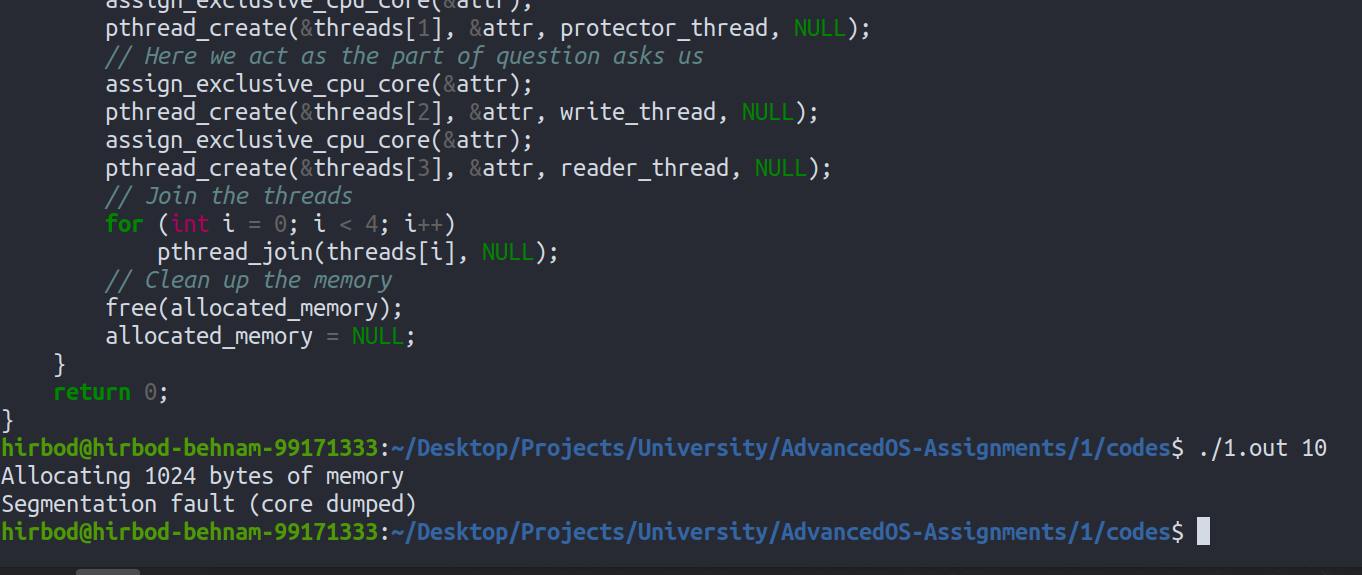
\includegraphics[scale=0.3]{pics/segfault3.png}
    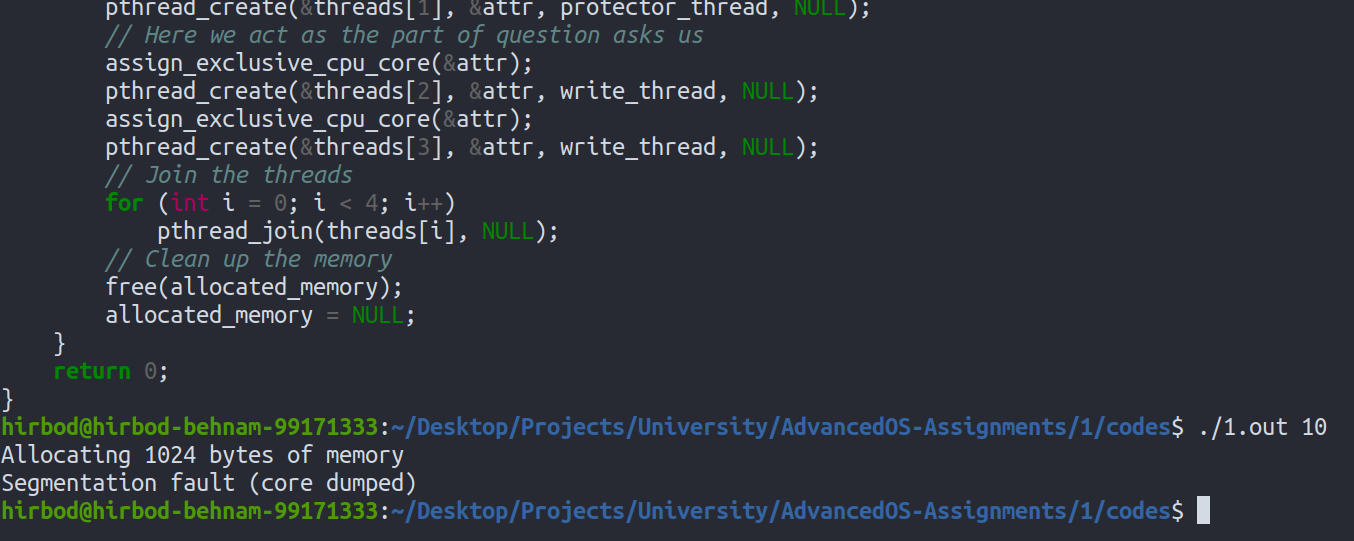
\includegraphics[scale=0.3]{pics/segfault4.png}
\end{figure}
همان طور که مشخص است باز هم
\lr{segfault}
می‌خوریم.
